\appendix


\section{Documentación para la reutilización del driver del codec}
	Para utilizar el driver hardware de sonido debes conocer los módulos necesarios y cómo conectarlos entre sí y como conectarlos a la FPGA, se aconseja mirar en paralelo la documentación del códec mencionado en la bibliografía.
	\subsection{Módulo Relojes}
		El codec necesita una serie de relojes que se generan a partir de uno de referencia (a partir de ahora clk) indicados en \cite{AK4565} MCLK, LRCK (el que dictará la frecuencia de muestreo), BCLK y CCLK, estos últimos pueden ser el mismo reloj, pero igual para tu aplicación tiene que ser distinto.
		Nosotros los generemos en fase para que no haya \emph{jitter} tan molesto en audio. Para ello lo realizamos con un sólo contador extrayéndo los bits necesarios tal y como se hace en \emph{I2SCLOCKS.vhd} \\

	Si la frecuencia con la que trabajases como reloj principal no es 50 MHz o si quisieras cambiar la frecuencia de algún reloj del codec por algún motivo concreto, este sería el módulo que habría que modificar.
		
	\paragraph{Temporización}
Una vez generados los relojes tendrás que trabajar sólo clk para que en los cambios de dominio entre datos gobernados por un reloj y otros datos gobernados por otro reloj no haya problemas, es decir si te interesa hacer una cosa cuando el reloj CCLK tenga un flanco negativo, toda tu aplicación tendrá que estar gobernada por clk y muestrear CCLK hasta que se produzca el cambio deseado y entonces actuar, con el reloj clk.
	
	\subsection{Módulo de Control}
		Este módulo configura al codec de audio para tenerlo operativo con lo mínimo tendrás que al menos escribir en dos registros, para escribir en los registros antes tendrás que poner a nivel bajo la señal CSN y a continuación mandar la palabra de 16 bits, donde 3 son para indicar escritura/lectura, 5 para la dirección (registro a escribir/leer) y los restantes 8 bits son el dato a escribir, y a continuación volver a nivel alto la señal CSN. \\
		Este ciclo lo tienes que repetir para cada palabra que quieras escribir:
		Por ejemplo si quieres selecionar que la entrada de audio es \emph{LINE} tendrás que escribir
		\begin{verbatim}
constant CDTI_data_input_sel : 
		STD_LOGIC_VECTOR (15 downto 0) := "0000100000000111";	
						  			       --"00001000_00000_111" -- Selects LINE
\end{verbatim}
	Y para selecionar el estandar I2S:
	\begin{verbatim}
constant CDTI_data_interface : 
STD_LOGIC_VECTOR (15 downto 0) := "0011110100010111"; 
						          --"00111101_00010_111" -- Selects I2S
\end{verbatim}
	
	Con estas dos palabras ya tendrías operativo el codec, pero hay otras configuraciones como \emph{fade-in} o \emph{fade-out} y otras muchas. Para mandar todas lo mejor es realizar una maquina de estados similar a la que se implementa en \emph{CONTROL.vhd} o modificar esta sustituyendo las palabras de configuración o añadiendo alguna más según se necesite.

	
	\subsection{Módulo I$^2$S}
	Este módulo se encarga de recoger los datos de audio del exterior y volcarlos en \emph{ADC$\_$RIGHT} y \emph{ADC$\_$LEFT}, que son dos puertos de 20 bits (resolución máxima del codec)
	y de coger los datos de tu aplicación en los puertos  \emph{DAC$\_$RIGHT} y \emph{DAC$\_$LEFT} y volcarlos al exterior de la forma adecuada.\\
	
	Tal y como se ha realizado este módulo te proporciona un dato nuevo en los dos puertos a la vez, cuando se produce un flanco negativo de LRCK y recoge los datos en los dos puertos en el mismo momento, por tanto no tienes que preocuparte de comunicarte con el módulo para entregar o recibir un dato, tú solo haz la funcionalidad.\\
	
	Si tu funcionalidad es sólo combinacional tan sólo escríbela, si tiene algún retardo entonces necesitarás temporizarla con clk muestreando LRCK, ejemplo:
	\begin{verbatim}
if  clk'event and clk = '1' then			
           ---- LRCK edge ----
          if LRCK /= lastLRCK then
					
                   lastLRCK <= LRCK;			
                           if LRCK = '0' then
                           
                                -- your application here!	
                                
                           end if;
           end if;
end if;
\end{verbatim}

	
 \newpage
	\subsection{Ilustración con una aplicación cualquiera}
		La más sencilla aplicación que puedes realizar debe tener estas entradas y salidas.\\
		\begin{figure}[H]
\begin{center}
	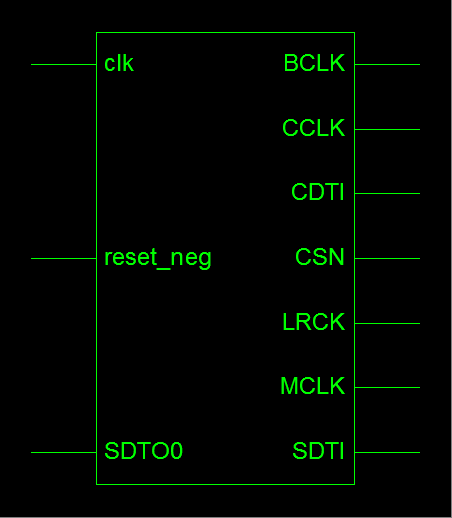
\includegraphics[width=0.4\textwidth]{./entity_fpga}
\caption{Minimas entradas y salidas de tu fpga}
\end{center}
\end{figure}
Y mirando el diagrama de bloques que lo componen:
\begin{figure}[H]
\begin{center}
	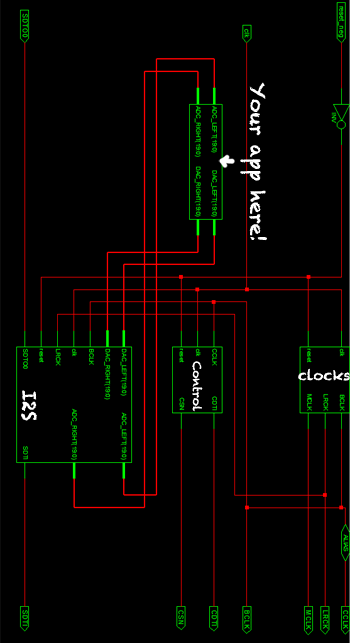
\includegraphics[scale=0.85]{./fig}
\caption{Bloques básicos y sus interconexiones para implementar una aplicación de audio}
\end{center}
\end{figure}
		

		

\section{Código}
